\documentclass[convert = false, tikz]{standalone}
\usepackage[utf8]{inputenc}
\usepackage{tikz}
\usetikzlibrary{automata, positioning, arrows, calc}

\usepackage{../../../../style_automata}

% arara: pdflatex
% arara: latexmk: { clean: partial }
\begin{document}
\tikzset{node distance=2.5cm}
\scalebox{0.8}{
    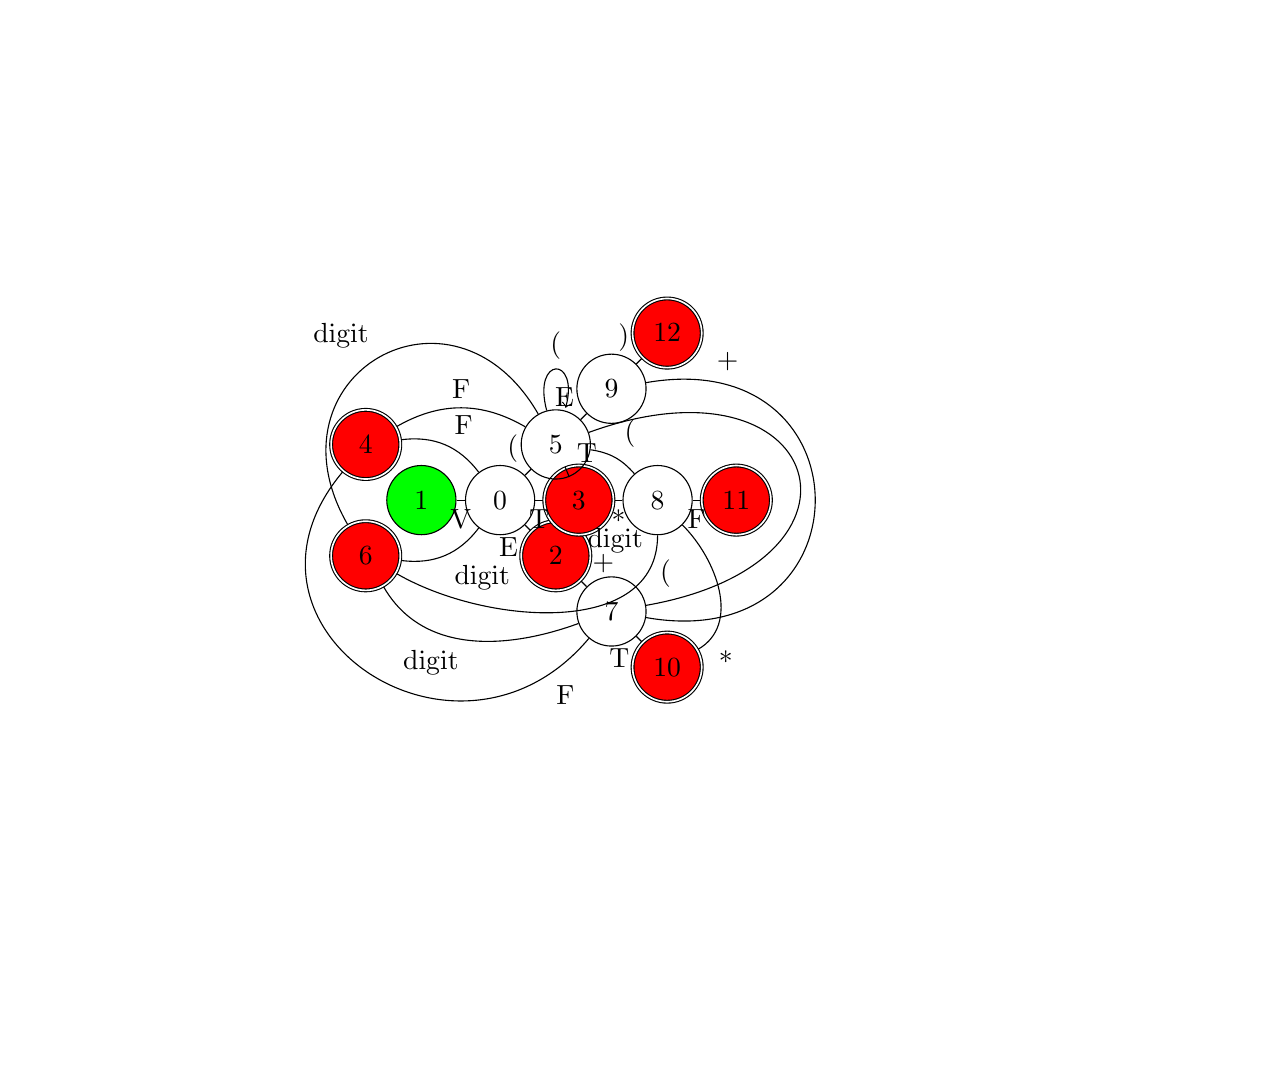
\begin{tikzpicture} 
        
        \node[state] (0) {0};
        \node[state, fill=green, left of=0] (1) {1};
        \node[state, accepting, fill=red, below right of=0] (2) {2};
        \node[state, accepting, fill=red, right of=0] (3) {3};
        \node[state, accepting, fill=red, above left of=1] (4) {4};
        \node[state, above right of=0] (5) {5};
        \node[state, accepting, fill=red, below left of=1] (6) {6};
        \node[state, below right of=2] (7) {7};
        \node[state, right of=3] (8) {8};
        \node[state, above right of=5] (9) {9};
        \node[state, accepting, fill=red, below right of=7] (10) {10};
        \node[state, accepting, fill=red, right of=8] (11) {11};
        \node[state, accepting, fill=red, above right of=9] (12) {12};
        
        \draw
        (0) edge[below] node{V} (1)
        edge[below left] node{E} (2)
        edge[below] node{T} (3)
        edge[above right, bend right=30] node{F} (4)
        edge[above left] node{(} (5)
        edge[below right, bend left=30] node{digit} (6)
        
        (2) edge[above right] node[pos=0.3]{+} (7)
        
        (3) edge[below] node{*} (8)
        
        (5) edge[above right] node{T} (3)
        edge[above, bend right=30] node{F} (4)
        edge[loop above] node{(} (5)
        edge[above left, out=120, in=120, looseness=2] node{digit} (6)
        edge[above left] node{E} (9)
        
        (7) edge[below right, out=-130, in=230, looseness=1.75] node[pos=0.1]{F} (4)
        edge[above left, out=10, in=20, looseness=3.5] node[pos=0.05]{(} (5)
        edge[below left, out=200, in=-60] node{digit} (6)
        edge[below left] node{T} (10)
        
        (8) edge[above right, bend right=20] node{(} (5)        
        edge[above left, out=-90, in=-30] node[pos=0.1]{digit} (6)        
        edge[below] node{F} (11)  
        
        (9) edge[above left] node{)} (12)
        edge[above right, out=10, in=-10, looseness=2.5] node[pos=0.1]{+} (7)
        
        (10) edge[below right, out=30, in=-45] node[pos=0.1]{*} (8)
        
        ;
        
        % Bottom left corner (x, y)
        \coordinate (A) at (-6,-7);

        % Top right corner (x, y)
        \coordinate (B) at (9.5,6); 
        
        \pgfresetboundingbox
        \path [use as bounding box] ($(A)$) rectangle ($(B)$);
        
    \end{tikzpicture}
}
\end{document}
    
    